{\let\clearpage\relax\chapter{Przedmioty zaawansowane}}
\section{AMO|EOPT|POPTY|TOP}
\subsection{Przedstawić metody minimalizacji funkcji bez ograniczeń oraz metody rozwiązywania zadań optymalizacji z ograniczeniami. Zdefiniować warunki konieczne i dostateczne optymalności ciągłych zadań optymalizacji z ograniczeniami i bez ograniczeń oraz warunki regularności.}
\textbf{Metody bez ograniczeń:}

\begin{description}
    \item[Poszukiwanie w kierunku]\mbox{}
    \begin{itemize}
        \item Metoda najszybszego spadku - Działanie metody najszybszego spadku jest bardzo podobne do metody gradientu prostego. Na samym początku algorytmu wybierany jest punkt startowy $\mathbf {x_{0}} \in D$. W punkcie tym obliczany jest antygradient $-\nabla f(\mathbf {x_{k}} )$ funkcji celu, który będzie stanowił kierunek poszukiwań w procedurze. Następny punkt jest obliczany według wzoru $\mathbf{x_{k+1}} = \mathbf{x_{k}}-\alpha_k\nabla f(\mathbf{x_{k}})$.\\Różnicą pomiędzy metodą najszybszego spadku a metodą gradientu prostego jest sposób wyszukiwania wartości $\alpha_{k}$ – dokonywana jest minimalizacja kierunkowa funkcji:\\ $f(\mathbf{x_{k}}-\alpha_k\nabla\mathbf{x_{k+1}}) = \min_{\alpha>0} f( \mathbf{x_{k}}-\alpha_k\nabla f(\mathbf{x_{k}}))$
        \item Metoda Newtona - połączenie idei iteracji i lokalnej aproksymacji liniowej. W tej metodzie iteracyjnej $x_{n+1}$ jest określone jako odcięta punktu przecięcia z osią x stycznej do krzywej y=f(x) w punkcie $(x_n,f(x_n))$.\\
        \begin{figure}[H]
        \centering
        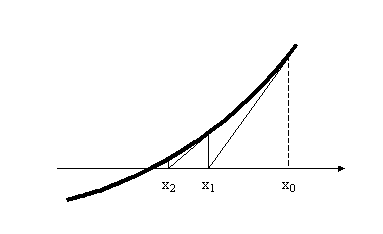
\includegraphics[width=0.5\linewidth]{fig/Metoda Newtona.png}
        \end{figure}
        \item Metody newtonowskie z aproksymacją różnicową - jest to metoda Newtona z tą różnicą, że równanie pochodnej funkcji minimalizowanej jest przybliżane z błędem rzędu O(h).\\ Aproksymacja ilorazem różnicowym w kierunku $w$ wygląda następująco:\\
        $F'(x)w\approx\frac{F(x+hw)-F(x)}{h}$
    \end{itemize}
    \item[Metody quasi-newtonowskie] - Metoda Quasi-Newtona może być używana, gdy obliczenie Hessianu (macierzy drugich pochodnych funkcji) wymaganego przez metodę Newtona jest trudne lub czasochłonne. Idea metody polega na przybliżeniu Hessianu lub jego odwrotności za pomocą pierwszych pochodnych.
    \item[Metody kierunków sprzężonych (Powella)] - Metoda Powella polega na poszukiwaniu minimum w kolejnych kierunkach bazowych. Kierunki bazowe w każdym cyklu poszukiwań ulegają modyfikacji, tak aby prowadziły one do szybszego znalezienia minimum, przy czym w kolejnych cyklach muszą być wzajemnie sprzężone. Metoda Powella pozwala odnaleźć minimum funkcji liniowo-kwadratowej w skończonej liczbie iteracji, w wyniku minimalizacji tej funkcji wzdłuż każdego kierunku tylko raz. Metodę Powella zastosować można nie tylko do funkcji będących formą kwadratową, ale także do dowolnych funkcji analitycznych, przyjmując, że w bliskim otoczeniu minimum można je przybliżyć formą kwadratową.
\end{description}

\textbf{Metody z ograniczeniami:}

Wiele metod bez ograniczeń można przystosować do optymalizacji z ograniczeniami (np. dodając do funkcji celu składnik kary za naruszenie ograniczeń).

\begin{description}
    \item[Metoda sympleks] - Składa się z dwóch podstawowych elementów:\mbox{}
    \begin{enumerate}
        \item Pierwszy, który osiągniemy dodając dodatkowe zmienne decyzyjne. W ten sposób dojdziemy do rozwiązania bazowego dopuszczalnego.
        \item Drugim elementem jest korekta przeprowadzonych już wcześniej iteracji rozwiązania bazowego dopuszczalnego do momentu, kiedy osiągniemy rozwiązanie optymalne, jeśli ono w ogóle istnieje.
    \end{enumerate}
    Istotą algorytmu simpleks jest badanie rozwiązań bazowych w postaci kanonicznej tak, aby znaleźć dowolne rozwiązanie programu, równocześnie sprawdzając czy jest ono optymalne. Jeżeli rozwiązanie nie jest optymalne, zaczynamy ponownie od znalezienia rozwiązania bazowego lepszego od poprzedniego. Kiedy stwierdzimy, że nie jesteśmy w stanie poprawić rozwiązania oznacza to, że rozwiązanie bazowe jest optymalne.
    \item[SLP] - Algorytm SLP polega na sprowadzeniu minimalizacji nieliniowej funkcji celu przy nieliniowych ograniczeniach do ciągu minimalizacji liniowej funkcji celu przy liniowych ograniczeniach (czyli tzw. zadania programowania liniowego - LP). Takie postępowanie jest szczególnie skuteczne dla funkcji słabo nieliniowych, ponieważ ich liniowe przybliżenie jest dość dokładne, a problem LP jesteśmy w stanie rozwiązywać bardzo szybko, nawet przy dużej liczbie zmiennych decyzyjnych.
\end{description}


\textbf{Warunek konieczny} optymalności:\\
$g(x^*) = \nabla f(x^*)=0$ - warunek I rzędu (stacjonarności), $x^*$ - minimum lokalne\\
$G^*(x^*) = \nabla^2f(x^*) = d^TH(x^*)d\geq{}0$ - warunek II rzędu 
\\\\

\textbf{Warunek dostateczny} lokalnego minimum:\\
$g(x^*) = \nabla f(x^*)=0$\\
$G^*(x^*) = \nabla^2f(x^*) = d^TH(x^*)d>0$ (warunek ściśle dodatniej określoności hesjanu - wypukłości w każdym kierunku)
\\\\

\textbf{Warunki regularności}
\begin{enumerate}
    \item Wszystkie funkcje ograniczeń $c_i$ są liniowe (Karlin).
    \item Wszystkie funkcje ograniczeń $c_i$ są funkcjami wypukłymi oraz istnieje taki punkt x, że $c_i(x) < 0$ dla wszystkich indeksów $i\in I$ (Slater).
    \item Gradienty wszystkich ograniczeń aktywnych ($\nabla c_i(\hat{x})$ dla $i\in A(\hat{x})$) są liniowo niezależne (Fiacco i McCormick).
\end{enumerate}

Spełnienie jednego z powyższych warunków wystarczy, aby punkt był optymalny. Jak jedno z ograniczeń nie jest spełnione, to możliwe jest inne.


\subsection{Opisać dualność zadań programowania liniowego i optymalizacji wypukłej. Zdefiniować odstęp dualności.}
Pomiędzy zadaniami dualnymi i prymalnymi zachodzą silne związki umożliwiające konstrukcje alternatywnych algorytmów rozwiązywania zadań programowania liniowego, jak również zmniejszenia nakładu obliczeń.

\begin{description}
    \item[Zadanie prymalne]: $\min{}_x c^Tx$\mbox{}\\
    Przy ograniczeniach:
    \begin{itemize}
        \item $Ax\geq b$
        \item $x\geq 0$
    \end{itemize}
    \item[Zadanie dualne:] $\max{}_\lambda b^T\lambda$\mbox{}\\
    Przy ograniczeniach:
    \begin{itemize}
        \item $A^T\lambda \leq c$
        \item $\lambda \leq 0$
    \end{itemize}
\end{description}

\begin{enumerate}
    \item Zamiast n-wymiarowego wektora zmiennych x mamy m-wymiarowy wektor zmiennych dualnych lambda (m - liczba ograniczeń pełnych zadania prymalnego).
    \item Wektor cen (c) modelu prymalnego staje się wektorem zasobów w zadaniu dualnym.
    \item Wektor zasobów (prawych stron ograniczeń liniowych) b staje się wektorem cen w zadaniu dualnym.
    \item W zadaniu prymalnym funkcja celu jest minimalizowana, w zadaniu dualnym maksymalizowana.
    \item Jeżeli w zadaniu prymalnym ograniczenia są typu równościowego to w zadaniu dualnym zmienne te są nieograniczone.
\end{enumerate}

Odstęp dualności - jest to różnica między wartością optymalną zadania dualnego i prymalnego.

\subsection{Przedstawić metody rozwiązywania zadań programowania kwadratowego z ograniczeniami. Omówić wykorzystanie zadań programowania kwadratowego w metodach ograniczonego obszaru zaufania i sekwencyjnego programowania kwadratowego.}

Zadania programowania kwadratowego sa drugim po zadaniach liniowych specyficznym typem zadań optymalizacji z ograniczeniami, dla których rozwinięto specjalne metody ich rozwiązywania. Zwykle przez pojęcie zadań programowania kwadratowego rozumie się zadania, w których funkcja celu jest kwadratowa, a ograniczenia liniowe.

Przykładowa funkcja celu: $\min{}_{x\in R^n} f(x) = \frac{1}{2}x^TGx+t^T$

\textbf{Metody rozwiązywania zadań programowania kwadratowego z ograniczeniami:}
\begin{description}
    \item[Ograniczenia równościowe] - \href{http://staff.uz.zgora.pl/acegiels/met-opt2020-r4.pdf}{Źródło}\mbox{}
    \begin{itemize}
        \item Metoda bezpośredniej eliminacji zmiennych - Metoda ta polega na wyznaczeniu m zmiennych z ograniczeń i wstawieniu ich do funkcji celu redukując w ten sposób wyjściowe zadanie do zadania minimalizacji bez ograniczeń funkcji n - m zmiennych.
        \item Metoda uogólnionej eliminacji - Metoda ta polega w istocie na tym, aby w eliminacji części zmiennych z ograniczeń równościowych Ax = b zadania wykorzystać rozkład spełniającego te ograniczenia wektora x na składową leżącą w ker A i składową leżącą w Im $A^T$.
    \end{itemize}
    \item[Ograniczenia nierównościowe] - Metoda zbioru ograniczeń aktywnych - Jej działanie jest podobne do działania metody Simplex. Metoda ta polega na włączaniu i usuwaniu ograniczeń ze zbiorów ograniczeń aktywnych (zbiór ograniczeń, na których krawędziach leży rozpatrywany punkt).
\end{description}

\textbf{Metoda obszaru zaufania}

Rozważmy problem minimalizacji funkcji skalarnej f(x) bez ograniczeń. Załóżmy, że punkt x znajduje się w n-wymiarowej przestrzeni i chcemy przejść z punktu x do punktu x takiego, że wartość funkcji celu f(x') < f(x). Metoda obszaru zaufania polega na przybliżaniu funkcji f inną, prostszą funkcją q, która w pewnym stopniu oddaje przebieg funkcji f w sąsiedztwie N punktu x. Sąsiedztwo to nazywamy obszarem zaufania. Krok próbny s jest wyliczany przez minimalizację w obszarze N. Tak zdefiniowany problem nazywamy podproblemem obszaru zaufania: $\min{}_s\{q(s),s\in N\}$.

Przejście z punktu x do punktu x + s następuje tylko jeżeli: $f(x+s) < f(x)$.

W innym przypadku punkt x pozostaje niezmieniony, obszar zaufania N ulega zawężeniu, a krok próbny zostaje powtórzony. 

W standardowej metodzie obszaru zaufania funkcja f jest aproksymowana przez wielomian drugiego stopnia q definiowany jako dwa pierwsze wyrazy szeregu Taylora. Sąsiedztwo N jest zazwyczaj sferyczne lub elipsoidalne.

\textbf{Sekwencyjne programowanie kwadratowe} jest jedną z najbardziej skutecznych metod numerycznego rozwiązywania zadań optymalizacji nieliniowej z ograniczeniami. Poniżej sformułowanie nieliniowego zadania optymalizacji, do którego stosujemy metodę SQP:

$\min_{x\in R^n} f(x)$\\
Przy ograniczeniach:
\begin{itemize}
    \item $c_E(x) = 0$
    \item $c_I(x) \leq 0$
\end{itemize}

SQP jest procedurą iteracyjną, która buduje model kwadratowy zadania nieliniowego w każdym punkcie iteracyjnym $x^k$, rozwiązuje podproblem kwadratowy, a następnie używa tego rozwiązania do konstrukcji kolejnego punktu iteracyjnego $x^{k+1}$. Jego konstrukcja jest realizowana w taki sposób, że ciąg $\{x^k\}_{k=1}^{+\infty}$ zbiega do lokalnego minimum zadania nieliniowego. W tym sensie jest podobna do metod Newtona i quasinewtonowskich do rozwiązywania układów równań nieliniowych. Jednakże obecność ograniczeń czyni analizę i implementację metod SQP znacznie bardziej skomplikowaną.

Metoda SQP rozwiązuje ciąg podproblemów optymalizacyjnych, każdy z nich optymalizuje model kwadratowy funkcji celu przy zlinearyzowanych warunkach ograniczających.

\section{ISR}
\subsection{Omówić kolejne poziomy reprezentacji ontologicznej stosowane w językach programowania robotów.}
Poziom ontologiczny języka programowania robotów wyznaczają przede wszystkim instrukcje ruchowe tego języka. Praktycznie we wszystkich językach instrukcje te odnoszą się albo do końcówki manipulatora, albo do jego złącz, a więc widać, że poziomy ontologiczne mogą być wymieszane w ramach jednego języka. Końcówką jest albo narzędzie, albo pewne miejsce charakterystyczne trzymanego przedmiotu. W przypadku narzędzi typu: aparaty spawalnicze, zgrzewarki lub pistolety lakiernicze rozkazy odnoszą się do pozycji części roboczej narzędzia. W przypadku chwytaków argumenty rozkazów ruchowych stanowią: pozycja punktu centralnego znajdującego się między szczękami lub, po uchwyceniu przedmiotu, jakaś jego część charakterystyczna, np. spód.

\begin{description}
    \item[Poziom stawów] - rusz się do pozycji w stawach
    \item[Poziom manipulatora] - rusz się do pozycji operacyjnej
    \item[Poziom obiektów] - połóż widelec na talerzu
    \item[Poziom zadania] - otwórz drzwi
\end{description}

\subsection{Omówić strukturę agenta upostaciowionego oraz sposób opisu jego działania.}
Agent upostaciowiony postrzega swoje środowisko przez receptory i oddziałuje na nie przez efektory. Funkcja przejścia stanowi program działania agenta. Struktura działania agenta odpowiada strukturze skończonego automatu (maszyna stanów).

Agent komunikuje się z rzeczywistymi efektorami i receptorami z wykorzystaniem ich wirtualnych odpowiedników, przechowując w ich dedykowanych buforach wartości zadane. Następnie rolą wirtualnych efektorów i receptorów jest translacja rzeczywistych wartości napędowych i czujnikowych do (i z) wartości rozumianych przez podsystem sterowania.

\begin{figure}[H]
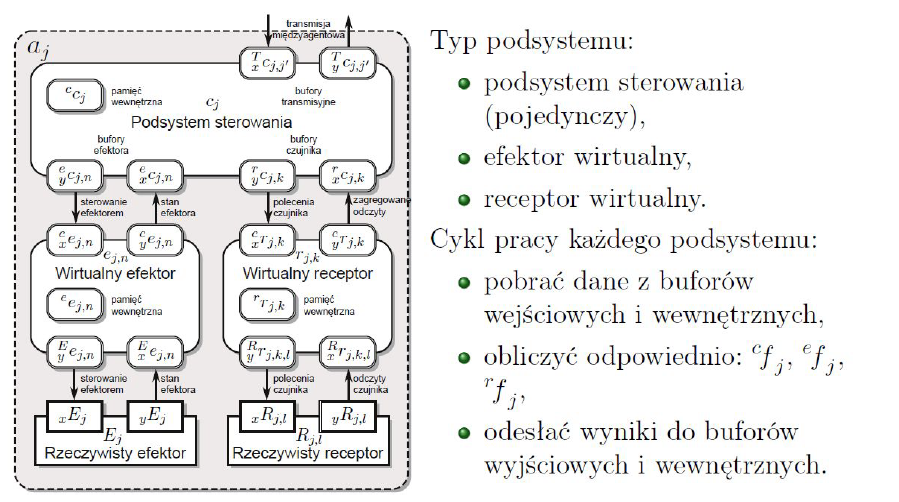
\includegraphics[width=\linewidth]{fig/Agent upostaciowiony.png}
\end{figure}


\subsection{Omówić podstawowe rodzaje map otoczenia i metody ich budowy.}
\textbf{Podstawowe rodzaje map:}
\begin{description}
    \item[Mapy metryczne] opisujące relacje geometryczne miedzy obiektami dzieli się na:\mbox{}
    \begin{itemize}
        \item Mapy rastrowe - najczęściej reprezentowane w postaci regularnej siatki (np. siatka zajętości) lub reprezentacje w postaci drzew (czwórkowych, ósemkowych).
        \item Mapy geometryczne - zwane też obiektowymi są zbudowane z obiektów (prymitywów) geometrycznych (punktów, linii, wielokątów...).
    \end{itemize}
    \item[Mapy topologiczne] są to grafy, w których węzły odpowiadają obserwowanym cechom (znacznikom), a łuki opisują związki między tymi cechami.
    \item[Mapy hybrydowe] to połączenie elementów geometrycznych i topologicznych.
    \item[Mapy kognitywne] zawierają dodatkowe, poza opisem geometrycznym i/lub topologicznym środowiska, informacje o obiektach, relacjach między obiektami oraz miejscach.
\end{description}

\textbf{Metody budowy map:}
\begin{description}
    \item[Metryczne] - budowane na podstawie pomiaru, rysunku CAR lub siatki zajętości.
    \item[Topologiczne] - grafy widoczności i diagramy Woronoja.
    \item[Obrazy RGBd] - RedGreenBlueDistance.
    \item[Mapy 3D] - postać chmury punktów.
\end{description}

\section{MI}
\subsection{Co to jest zmienna instrumentalna? Jakie warunki powinny one spełniać dla zapewnienia nieobciążonej estymaty? Jakie są typowe wybory zmiennej instrumentalnej?}
\textbf{Zmienna instrumentalna} jest to zmienna nieskorelowana z wyjściem y(t)
\begin{itemize}
    \item stosuje się ją do analizy modeli, których składnik losowy (patrz pytanie \ref{pyt:6}) nie jest zależny od zmiennych objaśniających model
    \item uogólnienie MNK
    \item metoda bezpośrednia w celu uniknięcia obciążenia estymaty
    \item dzięki metodzie zmiennych instrumentalnych, mimo tego, że zmienne objaśniające modelu są skorelowane ze składnikiem losowym, otrzymamy estymatę nieobciążoną (w przypadku MNK uzyskany estymator byłby obciążony)
    \item model w postaci $e=y-\Psi\hat{\Theta}$ mnożymy przez macierz zmiennych instrumentalnych W:\mbox{}\\
    $W^Te = W^Ty - W^T\Psi\hat{\Theta}$\\
    $\hat{\Theta} = (W^T\Psi)^{-1}W^Ty$
    \item Aby estymata była nieobciążona, liczba instrumentów jest równa liczbie zmiennych objaśniających (W ma taki sam wymiar jak $\Psi$)
\end{itemize}

W praktyce metoda zmiennych instrumentalnych polega na modyfikacji postaci modelu poprzez przemnożenie go przez macierz W skonstruowaną ze zmiennych instrumentalnych.

\textbf{Warunki zapewnienia nieobciążonej estymaty:}
\begin{itemize}
    \item nieskorelowane z n(k) - błąd losowy
    \item skorelowane z u(k) i $y_u(k)$ - zmienne objaśniające
\end{itemize}

\textbf{Wybór zmiennej instrumentalnej:}
\begin{itemize}
    \item można wykorzystać poprzednie (historyczne) wejścia jako zmienne instrumentalne:\mbox{}\\
    $w^T = (u(k-1-\delta)...(u(k-m-\delta)|u(k-d-1)...u(k-d-m))$
    \item wykorzystanie sygnału w oparciu o estymatę zakłócenia wyjścia:\mbox{}\\
    $w^T = (-h(k-1)...-h(k-m)|u(k-d-1)...u(k-d-m))$\\
    $h(k) = \hat{y_u}(j) = \Psi^T(k)\hat{\Theta}(k)$
\end{itemize}

\textbf{Podejście iteracyjne:}
\begin{enumerate}
    \item W pierwszej iteracji stosujemy zmienną instrumentalną w postaci sygnału wejściowego/
    \item W kolejnej iteracji na podstawie pierwszej iteracji wyniku oraz zmiennej instrumentalnej wygenerowanej w oparciu o estymatę niezakłóconego wyjścia wyliczamy kolejną estymatę parametrów.
    \item Powtarzamy krok 2. aż parametry się nie poprawią.
\end{enumerate}

\begin{description}
    \item[Estymator nieobciążony:]\mbox{}
    \begin{itemize}
        \item gdy obiekt jest odpowiednio pobudzony
        \item gdy jego wartość oczekiwana jest równą rzeczywistej wartości estymowanego parametru (tzn. jest najbardziej prawdopodobne, że właśnie ją otrzymamy)
        \item rząd modelu musi się zgadzać z rzędem identyfikowanego obiektu
    \end{itemize}
    \item[Estymator obciążony:]\mbox{}
    \begin{itemize}
        \item gdy występuje przesunięcie pomiędzy rzeczywistą wartością parametru, a wartością oczekiwaną estymatora
    \end{itemize}
\end{description}

\subsection{Jakie są różnice pomiędzy obserwatorem stanu i filtrem Kalmana? Przedstawić zasadę działania filtru Kalmana, zalety oraz ograniczenia.}
Filtr Kalmana może być użyty w roli obserwatora stanu (choć ma też inne zastosowania, np. nomen omen filtrowanie). Trudno zatem mówić o różnicach. Najczęściej na innych przedmiotach konstruowaliśmy obserwatory o stałym wektorze wzmocnień metodą lokowania biegunów. W ten sposób można dobrać obserwatora, który będzie zbiegał odpowiednio szybko do stanu obiektu pod warunkiem małego zaszumienia sygnałów – w przeciwnym wypadku będzie podążać za szumem. Filtr Kalmana jest przystosowany do działania w środowisku z zakłóceniami – lokuje swoje bieguny tak, by uzyskiwać statystycznie optymalne przewidywania.

Działanie filtra jest dwuetapowe (predyktor - korektor). Wpierw prognozowany jest stan jeden krok naprzód, potem prognoza ta jest korygowana w oparciu o nowy pomiar wyjścia. Stopień w jakim wykorzystywana jest informacja o aktualnym stanie wyjścia zależy od aktualizowanej na bieżąco macierzy wzmocnień K. Wyliczana jest na podstawie macierzy kowariancji stanów P (również aktualizowanej na bieżąco) – w taki sposób by minimalizować zależną od K i P wariancję błędu estymacji. W procesie stacjonarnym P i K dążą do wielkości ustalonych. Można zatem wyliczyć je a priori, co redukuje koszt obliczeniowy filtra.

\textbf{Zalety:}
\begin{itemize}
    \item rezultat statystycznie optymalny bez względu na obserwowalność i wykrywalność systemu, odporny na szumy, jak to tylko możliwe
    \item algorytm rekursywny – nie trzeba kumulować danych
\end{itemize}

\textbf{Wady:}
\begin{itemize}
    \item duży koszt obliczeniowy
    \item nie zawsze łatwo jest określić parametry zmiennych zakłócających (V), co prowadzi do trudności z inicjalizacją filtra
    \item działa dla liniowych procesów stacjonarnych przy założeniu, że wejście u(k) i stan x(k) to zmienne o rozkładzie gaussowskim (ale istnieją rozszerzenia znoszące te ograniczenia)
\end{itemize}

\subsection{Jak można wyznaczyć odpowiedź częstotliwościową systemów liniowych dla nieokresowych sygnałów testowych? Jakie są ich wady i zalety w stosunku do okresowych sygnałów testujących?}

Należy pobudzić takim sygnałem jakim się da (możliwie szeroko pobudzającym układ w dziedzinie częstotliwości), zebrać odpowiedź i wykonać transformatę Fouriera obu sygnałów. Ich stosunek odpowiada transmitancji widmowej obiektu - przekształcenie Fouriera stanowi
szczególny przypadek przekształcenia Laplace'a.

\textbf{Kryteria doboru sygnału wejściowego:}
\begin{enumerate}
    \item dobrze jest znać jego transformatę Fouriera
    \item musi być realizowalny przez obiekt
    \item powinien dobrze pobudzać różne częstotliwości
    \item im bardziej strome brzegi impulsu, tym większe wzbudzenie dla wyższych częstotliwości
    \item dla ustalonej amplitudy impulsu największa gęstość amplitudowa w widmie jest osiągana dla:\mbox{}
    \begin{itemize}
        \item skoku jednostkowego w przypadku niskich częstotliwości
        \item impulsów prostokątnych dla średnich i wysokich częstotliwości
    \end{itemize}
    \item sygnały te zapewniają najmniejszy błąd identyfikacji dla zaszumionych wejść
\end{enumerate}

W przypadku skoku jednostkowego, rampy, i niesymetrycznego impulsu trapezowego nie da się bezpośrednio wyznaczyć transformaty Fouriera. Można wzbudzić układ wiele razy tym samym sygnałem i uśrednić wyniki. Można też pobudzić wieloma różnymi sygnałami, ale wtedy uśredniać należy wyznaczone charakterystyki częstotliwościowe.

Skok jednostkowy i impuls prostokątny zapewniają najmniejszy błąd identyfikacji charakterystyk częstotliwościowych dla zaszumionych wyjść.

\begin{description}
    \item[Zalety:]\mbox{}
    \begin{itemize}
        \item jednoczesne pobudzenie wielu częstotliwości
        \item można sprawdzić wiele częstotliwości mieszcząc się w ograniczeniach obiektu (prędzej nam pozwolą puścić skok jednostkowy niż sinusoidę)
    \end{itemize}
    \item[Wady:]\mbox{}
    \begin{itemize}
        \item wyliczenie transformaty bywa kłopotliwe, niektóre sygnały jej nie mają
        \item istotne jest okienkowanie
        \item należy dobrze dobrać sygnał do badanego zakresu częstotliwości (aby dominował nad szumem)
        \item żeby dobrze dobrać sygnał warto byłoby już znać proces
    \end{itemize}
\end{description}


\section{MORO}
\subsection{Czym są i jak się rozwiązuje proste i odwrotne zagadnienie kinematyczne dla szeregowych łańcuchów kinematycznych?}
\begin{description}
    \item[Proste zagadnienie kinematyki] - mamy nastawy jointów i chcemy wyznaczyć pozycję chwytaka - \ref{pyt:22}
    \item[Odwrotne zagadnienie kinematyki] - posiadamy pozycję chwytaka i chcemy wyznaczyć ustawienie jointów - stosujemy przyrównanie macierzy oraz podstawianie, np.: $(T^0_1)^{-1}T^0_3 = T^1_3 = T^1_2T^2_3$
\end{description}

\subsection{Jaka jest ogólna struktura modelu dynamiki manipulatora szeregowego oraz jego napędu elektrycznego?}
\begin{description}
    \item[Struktura modelu dynamiki]: $\tau = M(\Theta)\ddot{\Theta}+B(\Theta,\dot{\Theta})+G(\Theta)$\mbox{}
    \begin{description}
        \item[$\tau$] - wektor momentów sił na każdym stawie
        \item[$M$] - macierz momentów bezwładności manipulatora
        \item[$B$] - wektor sił i momentów sił odśrodkowych i Coriolisa
        \item[$G$] - wektor sił i momentów sił grawitacji
    \end{description}
    \item[Moment wirnika zależny od prądu liniowego]: $M_W = M_B+M_\tau+M_{\mathrm{const}}$\mbox{}
    \begin{description}
        \item[$M_B$] - moment bezwładności $J\frac{d^2\Theta}{dt^2}$
        \item[$M_\tau$] - moment tarcia $B\frac{d\Theta}{dt}$
        \item[$M_{\mathrm{const}}$] - stały moment obciążenia
    \end{description}
\end{description}

\subsection{Omówić podstawowe metody generacji trajektorii dla manipulatorów.}
\textbf{Generacja trajektorii w przestrzeni złączy:}
\begin{itemize}
    \item wymaga mniej obliczeń online
    \item ciężka do przewidzenia trajektoria TCP (Tool Center Point)
    \item dobra do szybkich ruchów w nieograniczonej przestrzeni
    \item nie potrzeba obliczać OZK (odwrotne zadanie kinematyki)
\end{itemize}

\textbf{Generacja trajektorii w przestrzeni zadania:}
\begin{itemize}
    \item więcej obliczeń online
    \item możliwość unikania kolizji poprzez wyznaczenie trajektorii TCP
\end{itemize}

\textbf{Trajektoria z punktu do punktu w przestrzeni złącza:}
\begin{enumerate}
    \item wielomianowa 3-stopnia - 3 to najniższy stopień, gdyż to jest minimum by zadać początkowe i końcowe położenia oraz początkową i końcową prędkość. Cechuje się brakiem ciągłości funkcji przyspieszenia co powoduje szarpnięcie podczas sklejania trajektorii
    \item wielomianowa 5-stopnia - zapewnia ciągłość przyspieszenia, gładkie sklejenie prędkości
    \item LSPB - Linear Segments With Parabolic Blends (Symetryczny o trapezowym przebiegu prędkości)
    \item Bang-Bang specjalny przypadek LSPB bez stałego fragmentu przebiegu wartości prędkości - od płynnego przyspieszania bezpośrednio w płynne hamowanie (bez fazy ze stałą prędkością)
\end{enumerate}

\section{SST}
\textbf{Słowem wstępu}\\
Rozróżniamy dwa podstawowe rodzaje koordynacji: iteracyjną i periodyczną.

Koordynacja iteracyjna odpowiada jakby procesowi negocjacji pomiędzy decydentami, nazywanymi także jednostkami lokalnymi, z jednej strony, oraz koordynatorem (jednostka nadrzędna) z drugiej strony. Rezultatem tego iteracyjnego procesu ma być osiągnięcie stanu harmonii, w którym decyzje wszystkich ośrodków przekładają się na pożądane działanie systemu jako całości.

Na wykorzystaniu koordynacji iteracyjnej opierają się hierarchiczne metody optymalizacj: Metoda Bezpośrednia i Metoda Dualna, zwana także Metodą Cen.

Czynnik upływu czasu nie musi być w koordynacji iteracyjnej artykułowany, aczkolwiek w niektórych sytuacjach mechanizm tej koordynacji może być wykorzystany do sterowania systemów statycznych bądź systemów pracujących w stanie ustalonym, w oparciu o informacje pozyskiwane o aktualnych warunkach pracy tych systemów.

Jednym z zastosowań mechanizmu iteracyjnego Metody Cen może być sterowanie intensywnością transmisji źródeł ruchu w sieci danych.

Koordynacja periodyczna oparta jest o inną zasadę funkcjonowania: interwencje koordynatora modyfikujące działanie jednostek lokalnych mają miejsce w określonych odstępach czasu, pomiędzy tymi interwencjami jednostki lokalne realizują swoje zadania kierując się własnymi celami oraz wartościami instrumentów koordynujących przekazanych przez koordynatora.

W koordynacji periodycznej, stosowanej w złożonych układach sterowania i wspomagania decyzji, czynnik czasu odgrywa rolę podstawową. Jeśli przyjmiemy, że kolejne dyskretne chwile podejmowania decyzji $m_i$ przez i-tą jednostkę lokalną są określone wskaźnikiem czasu $k_l$ zaś wyróżniony podciąg tych chwil $\{k_l\}, l=1,...,...$, odpowiada kolejnym interwencjom koordynatora, to:

$m_l(k) = \mu (p(k_l),l_i(k))$ dla $k_l \leq k < k_{l+1}$

gdzie wielkość $p(k_l)$ oznacza wartość zestawu instrumentów koordynacji periodycznej ustaloną w chwili $k_l$, zaś $l_i(k)$ oznacza lokalną informację dostępną lokalnemu decydentowi w chwili k.

Ta ogólna zasada działania obecna jest w wielu systemach i organizacjach; postanowienia (wytyczne) podejmowane przez jednostkę nadrzędną są zmieniane, na ogół, w większych odstępach czasu niż decyzje określane lokalnie.

\subsection{Przedstawić zasadę działania Metody Bezpośredniej koordynacji iteracyjnej; podać jej podstawowe zalety i wady.}
\label{pyt:37}
Decydenci lokalni rozwiązują zadania cząstkowe modyfikowane przez koordynatora przy pomocy zmiennych koordynujących i przesyłają do koordynatora odpowiednie informacje; wartości zmiennych koordynujących są zmieniane do czasu osiągnięcia odpowiedniego warunku stopu (warunku koordynacji).

Na ogół dzieje się to tak, że koordynator proponuje wartości
zmiennych podsystemom, podsystemy optymalizują swoją użyteczność i zwracają do koordynatora jej wartość oraz w razie potrzeby inne informacje (np. wartość gradientu cząstkowego), koordynator znajduje nowe wartości zmiennych itd. aż ustali się równowaga.

\textbf{Zalety Metody Bezpośredniej:}
\begin{itemize}
    \item Mała wymiarowość zadań lokalnych; jest to podstawowa cecha metod hierarchicznych z koordynacją iteracyjną.
    \item Dla dopuszczalnych wartości zmiennych koordynujących zadania lokalne mają rozwiązania spełniające warunki nałożone na dostępne zasoby; inaczej mówiąc podczas procesu dochodzenia do optymalnego przydziału zasobów w każdej iteracji mamy do czynienia z dopuszczalnymi rozwiązaniami.
    \item Jeśli wyjściowe Zadanie Przydziału (ZP) ma rozwiązanie, to niezależnie od własności funkcji użyteczności oraz funkcji występujących w ograniczeniach, zadania lokalne $Zl_i$, i=1,..,N, a także zadanie ZK (Zadanie Koordynacji), są dobrze określone i zastosowanie Metody Bezpośredniej prowadzi do znalezienia rozwiązania zadania ZP.
\end{itemize}

\textbf{Wady Metody Bezpośredniej:}
\begin{itemize}
    \item Duża wymiarowość zadania ZK: liczba zmiennych koordynujących = N*J.
    \item Jeśli wskaźniki jakości w zadaniach lokalnych nie są ściśle wklęsłe lub funkcje występujące w ograniczeniach na zasoby nie są wypukłe, to możemy tracić różniczkowalność funkcji celu górnego poziomu i może ona być trudna w optymalizacji.
    \item Jeśli decydenci lokalni z jakiś powodów postanowią oszukiwać koordynatora, to mogą podawać zaniżone wartości lokalnych użyteczności odpowiadających proponowanym przydziałom zasobów, a także zawyżone wartości pochodnych odpowiadającym aktywnym ograniczeniem zasobów - w ten sposób mogą uzyskać przydział dodatkowych nienależnych im zasobów.
    \item Decydenci lokalni nie wnoszą żadnych opłat za użytkowanie zasobów, które są ograniczone: wada ta wiąże się z poprzednią i jest charakterystyczna dla tzw. gospodarki nakazowej.
    \item W przypadku pojawienia się w zadaniach lokalnych dodatkowych ograniczeń na wielkości $x_i$, na przykład w postaci $h_i(x_i)\geq 0$, może się łatwo zdarzyć, że trudno będzie koordynatorowi wyznaczyć zakres zmienności przydzielanych lokalnym jednostkom ilości zasobów, dla których zadania lokalne będą miały dopuszczalne rozwiązania.
\end{itemize}

\subsection{Przedstawić zasadę działania Metody Cen (Metody Zrównoważenia Interakcji) koordynacji iteracyjnej; podać jej podstawowe zalety i wady.}
Zamiast zadania prymalnego (pytanie \ref{pyt:37}) rozwiązuje się zadanie dualne. Mnożniki Lagrange'a odpowiadają cenom za poszczególne zasoby. ``Cena'' w tym kontekście oznacza zmniejszenie użyteczności podsystemu wskutek zużycia zasobu. Podsystemy starają się osiągnąć jak największą użyteczność skorygowaną o poniesiony koszt. Koordynator tak steruje cenami, żeby wyszło optymalnie.


\textbf{Zalety Metody Cen:}
\begin{itemize}
    \item Małą wymiarowość zadań lokalnych, podobnie jak w przypadku Metody Bezpośredniej; jest to podstawowa cecha metod hierarchicznych z koordynacją iteracyjną.
    \item Małą wymiarowość, równa J, wektora zmiennych koordynujących; jest to bardzo ważna zaleta Metody Cen; przypomnieć wypada, że w przypadku Metody Bezpośredniej liczba zmiennych koordynujących jest równa N*J.
    \item Zbiór punków dopuszczalnych każdego z zadań lokalnych jest bardzo prosty i niezależny od zmiennych koordynujących. W przypadku pojawienia się w zadaniach lokalnych dodatkowych ograniczeń na wielkości $x_i$, na przykład w postaci $h_i(x_i)\geq 0$, nie występują, w odróżnieniu od Metody Bezpośredniej, dodatkowe trudności.
    \item Jeśli zadanie koordynatora ma rozwiązanie w postaci wektora cen koordynujących p*, to punkt ten minimalizuje wypukłą funkcję dualną na zbiorze nieujemnych wektorów w przestrzeni $R_J$.
\end{itemize}

\textbf{Wady Metody Cen:}
\begin{itemize}
    \item Dla dopuszczalnych wartości zmiennych koordynujących zadania lokalne mogą mieć rozwiązania niespełniające ograniczeń nałożonych na dostępne zasoby; inaczej mówiąc podczas iteracyjnego procesu dochodzenia do optymalnego przydziału zasobów możemy mieć, i na ogół mamy, do czynienia z niedopuszczalnymi rozwiązaniami.
    \item Mogą nie istnieć wartości zmiennych koordynujących dla których spełniony zostaje warunek koordynacji, tj. może wystąpić luka dualności lub niemożność wybrania ze zbiorów rozwiązań zadań lokalnych punktów będących rozwiązaniami zadania PZ.
    \item Warunki wystarczające praktycznej stosowalności Metody Cen są bardzo wymagające; w podstawowej wersji tych warunków wymagana jest ścisła wklęsłość funkcji użyteczności i wypukłość funkcji określających zużycie zasobów.
\end{itemize}

\subsection{Opisać, na wybranym przykładzie, działanie układu hierarchicznego z koordynacją periodyczną.}
Koordynacja periodyczna: Jednostki lokalne kierują się swoimi celami oraz wartościami instrumentów koordynujących przekazanych przez koordynatora. Interwencje koordynatora modyfikujące ich działanie mają miejsce w określonych odstępach czasu.

Przykład koordynacji periodycznej - sterowanie zbiornikami retencyjnymi podczas przejścia fali powodziowej.

Operator zbiornika i, określający dyspozycje odpływu $q_i$ rozwiązuje zadanie $\min_{q_i} \max_t a_i(t)q_i(y)$ przy wymaganych ograniczeniach.

Koordynator w wyróżnionych momentach $t_i$ lub w miarę potrzeby (tzw. management by exception) określa, dla obydwu zbiorników, funkcje $a_i(t)$ w taki sposób, aby uzyskać możliwie małą kulminację w ważnym przekroju P, w którym występuje możliwość poniesienia istotnych strat powodziowych.


\section{TAP}
\subsection{Omówić układ regulacji wielopętlowej PID: zasady wyboru struktury połączeń, dobór nastaw regulatorów PI(D), odsprzęganie pełne i częściowe.}
Regulacja wielo-pętlowa PID stosowana jest do struktur wielowymiarowych ze słabymi interakcjami.


\begin{figure}[H]
\centering
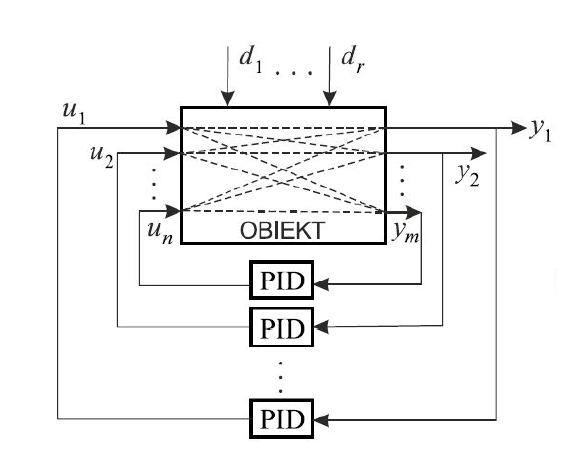
\includegraphics[width=0.5\linewidth]{fig/Struktura wielopętlowego PID.png}
\caption{Struktura wielopętlowego PID}
\end{figure}

\begin{figure}[H]
\centering
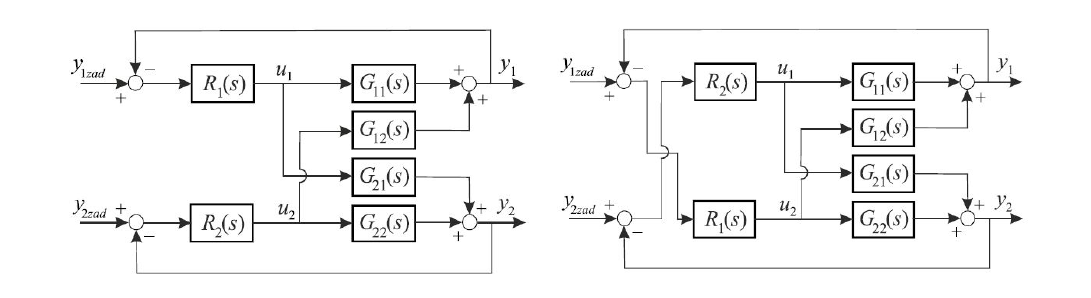
\includegraphics[width=\linewidth]{fig/Przykłady wielopętlowych PID.png}
\caption{Przykłady wielopętlowych PID}
\end{figure}

W powyższych strukturach występuje problem zjawiska ukrytego sprzężenia zwrotnego, w którym sygnał przebiega przez bloki: G12 -> y1 -> R1 -> G21 -> y2 -> R2 -> G12 ... (w przypadku struktury 1-1/2-2 - pierwszy przykład).

\textbf{Wybór struktury połączeń} - Metoda RGA

Rozważamy dwie struktury:
\begin{enumerate}
    \item Wszystkie pętle regulacyjne rozwarte (regulatory na ``manual'', sterowania ustalone),
    \item Pętla $u_j -> y_i$ rozwarta, wszystkie pozostałe regulatory na ``automatic'' (pętle zamknięte, regulatory stabilizują pozostałe wyjścia)
\end{enumerate}

W każdej z tych sytuacji wyznaczane są wzmocnienia w torze $u_j -> y_i$, podając skok na wejście $u_j$ i czekając na ustalenie się wyjść:
\begin{enumerate}
    \item Pętle regulacyjne rozwarte:\mbox{}
    $k_{ij} = \left(\frac{\partial y_i}{\partial u_j}\right)_{u_k=\mathrm{const}\:\mathrm{dla}\: k\neq j}$
    \item Pętla $u_j->y_i$ rozwarta, wszystkie pozostałe pętle regulacji zamknięte:\mbox{}
    $k_{ij}^{c;} = \left(\frac{\partial y_i}{\partial u_j}\right)_{y_k=\mathrm{const}\:\mathrm{dla}\: k\neq i}$
\end{enumerate}

Względne wzmocnienie w torze $u_j->y_i$:\mbox{}
$\lambda_{ij} = \frac{k_{ij}}{k_{ij}^{cl}}$

\textbf{Podstawowe zasady wyboru połączeń w strukturze wielopętlowej:}
\begin{enumerate}
    \item Nie należy wybierać połączeń, którym odpowiadają ujemne wartości $\lambda_{ij}$ (zmiana znaku pętli sprzężenia $y_i->u_j$ po zamknięciu/otwarciu innych pętli!),
    \item Należy wybierać połączenia, którym odpowiadają wartości $\lambda_{ij}$ bliskie 1 (zamykanie/otwieranie innych pętli niewiele wpływa na pętlę $y_i->u_j$). 
\end{enumerate}

\textbf{Metody doboru nastaw regulatorów PI(D):}
\begin{description}
    \item[Metody heurystyczne:] Dobór nastaw PI(D) dla transmitancji głównych SISO $G_{jj}(s)$, a następnie korekta nastaw metodą prób i błędów, na początku z reguły stłumienie (detuning: zmniejszanie wzmocnień, zwiększanie czasów całkowania, itp.) - aż do osiągnięcia założonego celu:\mbox{}
    \begin{itemize}
        \item formalnego, np. odpowiednia wartość kryterium (metoda BLT Luybena),
        \item bardziej intuicyjnego -odpowiednie przebiegi odpowiedzi na skoki zakłóceń i/lub wartości zadanych.
    \end{itemize}
    \item[Metoda optymalizacji parametrycznej:] Nastaw regulatorów PI(D) - modelujemy układ regulacji i optymalizujemy nastawy wg wybranego kryterium, np. ISE. Wskazane dobre modelowanie obiektu - np. nieliniowe modelowanie obiektu w pętli symulacyjnej, a liniowy model uproszczony jedynie do wstępnego doboru nastaw (punktu startowego optymalizacji).
    \item[Inne:] Istnieje w literaturze szereg propozycji metod doboru nastaw, ale nie zdobyły one szerszego uznania i zastosowania.
\end{description}

\textbf{Odsprzęganie dynamiczne (pełne)}:

Wprowadzone zostają bloki pośredniczące, łączące sygnał R1 z G22 oraz R2 z G11 (w przypadku połączenia 1-1/2-2). Bloki te nazywają się kolejno D21 oraz D12.

Odprzęganie może skutecznie kompensować interakcje przy nadążaniu za wartościami zadanymi i tłumieniu zakłóceń działających na wyjściu obiektu - może nawet pogorszyć tłumienie zakłóceń działających interaktywnie.
\\\\

Warunki idealnego odsprzęgania:\mbox{}\\
$G_{21}(s)U_{R1}(s)+G_{22}(s)D_{21}(s)U_{R1}(s)=0$\\
$G_{12}(s)U_{R2}(s)+G_{11}(s)D_{12}(s)U_{R2}(s)=0$
\\\\

Stąd transmitancje idealnych bloków odsprzęgających:\\
$D_{21}(s)=-\frac{G_{21}(s)}{G_{22}(s)}$,\\
$D_{12}(s)=-\frac{G_{12}(s)}{G_{11}(s)}$.

W odsprzęganiu nierealizowalne są elementy:
\begin{itemize}
    \item opóźnienia: pozbywamy się $e^{Ts}$ z licznika,
    \item bieguny niestabilne: pozbywamy się biegunów z prawej półpłaszczyzny układu współrzędnych z mianownika.
\end{itemize}

\textbf{Odsprzęganie częściowe:}
Jeśli jedna interakcja jest silna (istotna), a druga słaba (mniej istotna), to można zastosować odsprzęganie częściowe (jednokierunkowe).

Wadą układów regulacji z odsprzęganiem jest wrażliwość na błędy modelowania i na zmiany parametrów obiektu - tym większa, im bardziej złożony układ odsprzęgający.

Konsekwencją układu regulacji wielopętlowej jest to, że strojenie regulatorów jest trudniejsze, bowiem nie może być dokonywane niezależnie, a odłączanie/dołączanie poszczególnych pętli może nawet zdestabilizować pozostałe.

\subsection{Przedstawić zasadę regulacji predykcyjnej (MPC), sformułowanie wielowymiarowych algorytmów wyznaczania sterowań numerycznego i analitycznego (prawa regulacji), scharakteryzować krótko podstawowe algorytmy wielowymiarowe z liniowym modelem procesu.}
\textbf{Regulacja predykcyjna MPC:}
\begin{itemize}
    \item technika silnie oparta na modelu obiektu, wymagająca znacznie większego nakładu obliczeń niż algorytmy PID,
    \item w sposób naturalny uwzględnia ograniczenia można je stosować do obiektów wielowymiarowych z silnymi interakcjami, również przy nierównej liczbie wejść sterujących i wielkości regulowanych do obiektów o trudnej dynamice.
\end{itemize}

Optymalizujemy przyrosty sterowania na horyzoncie sterowania (od chwili k do k+Nu-1). Optymalizacja ma na celu zminimalizowanie błędu przy jednoczesnym zachowaniu możliwie niewielkich zmian sterowania (kara za zmianę sterowania). Estymujemy wyjścia na horyzoncie predykcji.

\begin{equation}
   \min_{\Delta u(k|k),...,\Delta u(k+N_u-1|k)} \left\{ J(k) = \sum_{p=1}^N \left\| \left[ y^{zad}(k+p|k) - y(k+p|k) \right]\right\|^2 + \lambda \sum_{p=0}^{N_u-1} \left\| \Delta u(k+p|k) \right\|^2 \right\} 
\end{equation}

Z ograniczeniami na minimum i maksimum sygnału $u(k+p|k)$, $\Delta u(k+p|k)$ oraz $y(k+p|k)$.

\textbf{Analityczne prawo regulacji}\\
Macierz dynamiczna “M” - zależy od konkretnej implementacji - oraz macierze diagonalne $\Psi$ oraz $\Lambda$ o wymiarowościach $(n_y\cdot N) \times (n_y\cdot N)$ i $(n_u\cdot N_u) \times (n_u\cdot N_u)$, odpowiednio ($n_u=\dim u$ jest liczbą sterowań obiektu).

$K = [M^T\Psi M + \Lambda]^{-1}M^T\Psi$

Wektor optymalnych przyrostów sterowań:

$\Delta \hat{U}(k) = K[Y^{zad}(k)-Y^0(k)]$
\\\\

Prawo regulacji MPC bez ograniczeń:

$\Delta u(k) =\Delta \hat{u}(k|k) = \bar{K}_1[Y^{zad}(k)-Y^0(k)]$\\
gdzie:\\
$Y_0$ - odpowiedź swobodna\\
$\bar{K}_1$ = macierz o wymiarze $n_u\times (n_y\cdot N)$ złożona z pierwszych $n_u$ wierszy macierzy $K$.

\textbf{Numeryczne prawo regulacji}

Przyjmując:\\
$x = \Delta U(k)$\\
$H = 2(M^T\Psi M + \Lambda)$\\
$f = -2M^T\Psi(Y^{zad}(k)-Y^0(k))$\\
$A = [-J\:;\:J\:;\:-M\:;\:M]$\\
$b = [-U_{min} + U(k-1)\:;\:U_{min} - U(k-1)\:;\:-Y_{min} + Y^0(k)\:;\:Y_{min} - Y^0(k)]$\\
$J = [I\:0\:0\:;\:I\:I\:0\:;\:I\:I\:I]$\\
dostajemy zadanie optymalizacji regulatora MPC w postaci standardowej dla zadania programowania kwadratowego:
\begin{equation}
    \min \left\{ J(x) = \frac{1}{2}x^THx+f^Tx\right\}
\end{equation}

Uwaga: macierze H i A są stałe i wyznaczamy je off-line, wektory f i b zależą od $Y^0(k)$ i $U(k-1)$ - wyznaczamy je on-line w każdym kroku k regulatora.

\textbf{Scharakteryzować krótko podstawowe algorytmy wielowymiarowe z liniowym modelem procesu:}
\begin{description}
    \item[DMC] - M na podstawie odpowiedzi skokowej,
    \item[GPC] - M na podstawie wyznaczenia odpowiedzi skokowej z modelu różnicowego (y(k) = 0 dla k < 0, u(k) = 1 dla k >= 0),
    \item[MPCS] - M wyznaczamy na podstawie parametrów równań stanu (macierze A, B i C).
\end{description}

\subsection{Omówić podstawowe algorytmy nieliniowej regulacji predykcyjnej z numerycznymi zadaniami optymalizacji sterowań (MPC-NO, MPC-NPL), oraz szybki algorytm bazujący na liniowych prawach regulacji.}
\begin{description}
    \item[NO (Non-linear Optimization)] - w każdej iteracji optymalizujemy sterowanie na podstawie modelu nieliniowego
    \item[NPL (Nieliniowa Predykcja trajektorii początkowej i Linearyzacja modelu dla optymalizacji)] - w każdej iteracji najpierw linearyzujemy, a potem optymalizujemy na podstawie modelu liniowego (szybsze, mniej dokładne)
    \item[GPC] - najpierw linearyzujemy model, potem w każdej iteracji optymalizujemy
    \item[NMPC] - szybki algorytm bazujący na modelach rozmytych T-S
(najszybsze, najmniej dokładne)
\end{description}

\textbf{Opis algorytmów:}

\begin{description}
    \item[NO]\mbox{}
    \begin{itemize}
        \item pełna nieliniowa regulacja MPC, z predykcją całej trajektorii wyjść opartą na modelu nieliniowym
        \item w każdym kroku predykcja trajektorii wyjść obliczanych modelem nieliniowym wykonywana jest wielokrotnie, dla każdego kolejnego wektora zmiennych decyzyjnych wyznaczanych przez algorytm optymalizacji
        \item mamy nieliniowy model procesu (w postaci równania różnicowego lub w postaci nieliniowych równań stanu) i na jego podstawie wykonywane jest zadanie optymalizacji dynamicznej regulatora MPC
        \item predykcje wyjść liczone są z użyciem nieliniowego modelu procesu, zaś u(k-1|k) = u(k-1)
        \item rekurencyjne obliczanie predykowanej trajektorii wyjść dla każdej aktualnej trajektorii sterowań
        \item estymacja stanu procesu nieliniowego: mamy nieznany dokładnie nieliniowy proces i estymujemy stan na podstawie modelu (albo metodą rozszerzonego filtru kalmana, albo rozszerzonego obserwatora Luenberga)
    \end{itemize}
    \item[NPL] - w każdej iteracji algorytmu NPL powtarzana jest sekwencja czynności:\mbox{}
    \begin{itemize}
        \item linearyzacja modelu nieliniowego (nieliniowy)
        \item wyznaczenie macierzy dynamicznej (zlinearyzowany z punktu poprzedniego)
        \item obliczenie odpowiedzi swobodnej (nieliniowy)
        \item sformułowanie zadania optymalizacji kwadratowej
        \item wyznaczenie sterowania
    \end{itemize}
    \item[FMPC]\mbox{}
    \begin{enumerate}
        \item Regulator nieliniowy rozmyty T-S DMC analityczny\mbox{}
        \begin{itemize}
            \item Reguła wnioskowania: każda reguła R' odpowiada jednemu podobszarowi A, gdzie zaprojektowano regulator DMC
            \item Wnioskowanie rozmyte - nieliniowe uśrednianie z wagami w'(k) odpowiadającymi sile aktywności poszczególnych reguł
        \end{itemize}
        \item Nieliniowy analityczny regulator GPC rozmyty T-S: z lokalnymi liniowymi prawami regulacji GPC stanowiącymi następniki reguł wnioskowania (wnioskowanie rozmyte jak w nieliniowym DMC wyżej)
        \item Nieliniowy analityczny regulator MPCS rozmyty T-S: z lokalnymi liniowymi prawami regulacji MPCS stanowiącymi następniki reguł wnioskowania (wnioskowanie rozmyte jak poprzednio)
    \end{enumerate}
\end{description}

\section{TST}
\subsection{Przedstawić opisowo typowe wymagania jakie musi spełniać dobrze zaprojektowany system regulacji. Powiązać je z wymaganiami dotyczącymi transmitancji składających się na podstawowe równanie systemu regulacji.}
Generalnie układ jest stabilny jezeli jego stan/odpowiedź nie robiega się do nieskończoności. Dokładniejsze definicje stabilności są bardzo różne. Można podzielić je na dwie kategorie określające:
\begin{enumerate}
    \item stabilność ze względu na warunki początkowe (stan układu nie rozbiega się po wychyleniu ze stanu początkowego przy braku sygnału wejściowego),
    \item stabilność ze względu na wymuszenie (odpowiedź układu nie rozbiega się w wyniku podania dowolnego ograniczonego sygnału wejściowego)
\end{enumerate}

\textbf{Stabilność w sensie Lapunowa:}\\
Układ jest stabilny w punkcie $x_e$, jeżeli dla dowolnie wybranej odległości $\varepsilon$ od stanu $x_e$ istnieje taka odległość $\delta$, że dla dowolnego wychylenia ze stanu $x_e$ nie większego od $\delta$, stan układu nie odejdzie od $x_e$ dalej niż na $\varepsilon$.\\
Innymi słowy: dla żadnego wychylenia ze stanu $x_e$ stan układu nie oddala się nieskończenie od $x_e$. Nie musi jednak do niego wracać, a koniec końców może znaleźć się dalej niż wychylono $\varepsilon>\delta$.

Własność ta może być lokalna albo globalna. Globalnie: dla żadnego wychylenia, lokalnie: dla żadnego wychylenia mieszczącego się w pewnych granicach.

\textbf{Układ niestabilny:}\\
Układ jest niestabilny w punkcie $x_e$ jeżeli dla dowolnie małego wychylenia ze stanu $x_e$ stan oddala się nieskończenie od $x_e$.

\textbf{Układ zbieżny:}\\
Układ jest zbieżny w punkcie $x_e$ jeżeli dla dowolnego wychylenia $\delta$ stan układu powraca do $x_e$. Ale zanim tam zbiegnie może dowolnie wariować i osiągać wartości dalsze niż $\delta$.

\textbf{Układ stabilny asymptotycznie:}\\
Układ jest stabilny asymptotycznie jeżeli jest stabilny i zbieżny. Innymi słowy: od razu dąży do wartości $x_e$.

Globalnie asymptotycznie stabilny: istnieje tylko jeden punkt równowagi.

\textbf{Stabilność ze względu na wymuszenie:}
\begin{description}
    \item[Układ stabilny] jest jeżeli dla dowolnego przebiegu sygnału wejściowego osiągającego skończone wartości odpowiedź układu nie będzie rozbiegać się do nieskończoności.
    \item[Układ niestabilny] jest wtedy gdy układ nie jest... stabilny.
\end{description}

\textbf{Nieskończona odpowiedź:}\\
W rzeczywistych układach odpowiedź albo ucieczka od stanu początkowego nigdy nie jest nieskończona, ponieważ żaden rzeczywisty układ nie jest w nieograniczonym zakresie liniowy. Obrazowo mówiąc: w rzeczywistości prędzej układ ulegnie zniszczeni niż osiągnie wartości nieskończone. Warto na to zwrócić uwagę, bo zwykle nie jest to ujęte w modelu matematycznym.

\textbf{Algebraiczne kryteria stabilności:}\\
Kryteria algebraiczne określające stabilność układów liniowych wyprowadzone są z twierdzenia o stabilności: aby układ liniowy był globalnie asymptotycznie stabilny wystarczy żeby wszystkie pierwiastki równania charakterystycznego układu (mianownik transmitancji całego układu = 0) znajdowały się w lewej półpłaszczyźnie zmiennej zespolonej s. Dzieje się tak, ponieważ członom typu $\frac{1}{s-a}$ transmitancji odpowiadają wyrazy typu $e^{at}$ w dziedzinie rzeczywistej (i znajdą się wobec tego w sygnale wyjściowym). Jeżeli a jest urojone to wystąpią oscylacje. Oscylacje te będą gasnące tylko jeżeli część rzeczywista pierwiastka a (odpowiadająca eksponencjalnej obwiedni sinusoidy) będzie ujemna.

\textbf{Kryterium Hurwitza:}\\
Równanie charakterystyczne układu (o współczynnikach rzeczywistych):\\
\begin{equation}
    a_ns^n+a_{n-1}s^{n-1}+...+a_1s + a_0 = 0
\end{equation}
\begin{description}
    \item[Warunek konieczny] globalnej stabilności asymptotycznej układu liniowego: wszystkie współczynniki równania muszą być tego samego znaku.
    \item[Warunek wystarczający]: wszystkie wyznaczniki $\Delta_i$ są większe od zera.
\end{description}

\textbf{Kryterium Routha:}\\
\begin{description}
    \item[Warunek konieczny] globalnej stabilności asymptotycznej układu liniowego: wszystkie współczynniki równania muszą być tego samego znaku.
    \item[Warunek wystarczający]: wszystkie elementy pierwszej kolumny tablicy Routha mają ten sam znak.
\end{description}
Liczba zmian znaków w pierwszej kolumnie tablicy równa jest liczbie pierwiastków w prawej półpłaszczyźnie.

\textbf{Częstotliwościowe kryteria stabilności}

\textbf{Kryterium Nyquista:}\\
Pozwala na określenie stabilności układu zamkniętego (ze sprzężeniem zwrotnym) na podstawie badania charakterystyki amplitudowo-fazowej układu otwartego.

Jeżeli układ otwarty jest stabilny to układ zamknięty będzie stabilny wtedy i tylko wtedy, gdy charakterystyka amplitudowo-fazowa układu otwartego nie obejmuje punktu $(-1,j_0)$ na płaszczyźnie zespolonej. Gdy charakterystyka przechodzi przez ten punkt to układ jest na granicy stabilności.

Punkt ten jest istotny, ponieważ odpowiada częstotliwości najbardziej krytycznej dla układu, a mianowicie takiej dla której sygnał na końcu toru sprzężenia zwrotnego będzie przesunięty w fazie o $\pi$.

\textbf{Wykresy Bodego:}\\
\begin{description}
    \item[Zapas modułu] jest to współczynnik przez jaki należy przemnożyć wzmocnienie układu przy niezmienionym argumencie transmitancji widmowej układu otwartego, aby doprowadzić układ do granicy stabilności.
    \item[Zapas fazy] mierzony w stopniach określa wartość zmiany argumentu transmitancji widmowej układu otwartego potrzebny, aby doprowadzić układ do granicy stabilności.
\end{description}

Z kryterium Nyquista sprawa jest w sumie odrobinę bardziej skomplikowana, ale nie ma co się w to zagłębiać. Dodać wypadałoby badanie stabilności w przypadku układów dyskretnych opisanych równaniami stanu. Wówczas wystarczy sprawdzić promień spektralny macierzy dynamiki układu (jeśli któryś jest większy niż 1 to na związanym z nim kierunkiem własnym układ jest niestabilny). Widmo - pierwiastki równania det(zI-A)=0. Co do stabilności w dziedzinie transmitancji: w czasie ciągłym bieguny układu muszą być w lewej półpłaszczyźnie, w czasie dyskretnym – wewnątrz koła jednostkowego.

\textbf{Wszystkie wymagania:}
\begin{enumerate}
    \item Stabilność
    \item Zapas fazy i modułu
    \item Realizowalne i bezpieczne wartości i przyrosty sygnałów (ograniczenia)
    \item Spełnienie wymagań dotyczących jakości regulacji (metryki jakości) - np. czas potrzebny układowi do stabilizacji lub maksymalne przeregulowania
    \item Odporność na zakłócenia
\end{enumerate}

\textbf{Wymagania transmitancji:}\\
Transmitancje w czasie ciągłym muszą mieć bieguny w lewej półpłaszczyźnie (czyli Re(s)) < 0).\\
Transmitancje w czasie dyskretnym muszą mieć bieguny wewnątrz koła jednostkowego.


\subsection{Podać definicję stabilności „ograniczone wejście-ograniczone wyjście” (ang. BIBO stability). Jakie warunki gwarantują BIBO stabilność stacjonarnego układu liniowego dla każdego warunku początkowego. Rozpatrzyć układy z czasem ciągłym i dyskretnym.}

System opisany równaniem $y(t)=H(q)u(t)$ jest stabilny w sensie BIBO, jeżeli dla każdego ciagu sterowań spełniających warunek $|u(t)|\leq c_0$ spełniony jest warunek $|y(t)|\leq c_1$, gdzie $c_0,c_1<\infty$.

Innymi słowy układ jest BIBO stabilny jeżeli jego odpowiedź na ograniczony sygnał wejściowy jest również ograniczona.

Warunki:
\begin{description}
    \item[Czasu ciągłego (konieczny i wystarczający):] $\int_{-\infty}^\infty |h(t)\mathrm{d}t|=\|h\|_1<\infty$
    \item[Czasu dyskretnego (wystarczający):] $\sum_{n=-\infty}^\infty |h[n]| = \|h\|_1<\infty$
\end{description}


\subsection{Sformułować zadanie wyznaczenia optymalnego regulatora liniowo-kwadratowego (zadanie LQR). Omówić wybór parametrów wskaźnika jakości w tym zadaniu. Podać postać rozwiązania tego zadania. Rozpatrzyć układy z czasem ciągłym i dyskretnym.}
Regulacja liniowo-kwadratowa dla obiektu liniowego w przestrzeni stanu polega na doborze sterowań optymalizujących pewną kwadratową funkcję kosztu zdefiniowaną na sygnałach sterujących i wyjściowych. Funkcja ta zapisana jest w postaci całki dla systemu ciągłego lub w postaci sumy dla systemu dyskretnego.

\textbf{LQR w czasie ciągłym}

Układ liniowy określony równaniem: $\dot{x}=Ax+Bu$\\
Funkcja kosztu: $J=\int_0^\infty \left( x^TQx + u^TRu \right)dt$\\
Sterowanie ze sprzężeniem: $u=-Kx$\\
Dla K równego: $K=R^{-1}B^TP$\\
Z P wyznaczanym z równania algebraicznego Riccatiego dla czasu ciągłego:\\
$A^TP+PA-PBR^{-1}B^TP+Q=0$


\textbf{LQR w czasie dyskretnym}

Układ liniowy określony równaniem: $x_{k+1}=Ax_k+Bu_k$\\
Funkcja kosztu: $J=\sum_{k=0}^\infty \left( x_k^TQx_k + u_k^TRu_k \right)$\\
Sterowanie ze sprzężeniem: $u_k=-Fx_k$\\
Dla F równego: $F=\left(R+B^TPB\right)^{-1}B^TPA$\\
Z P wyznaczanym z równania algebraicznego Riccatiego dla czasu dyskretnego:\\
$P=Q+A^T\left(P-PB\left(R+B^TPB\right)^{-1}B^TP\right)A$


